\section{System Overview}
\label{sec:overview}

\subsection{Architecture at a Glance}
\label{sec:arch-glance}

The system is organized as a vertical stack of layers. Lower layers provide
services to higher layers; no layer reaches past its immediate neighbor.
A problem in one layer does not propagate downward, and upper layers can be
developed, replaced, or disabled independently of the foundation beneath them.
The AI layer, for example, sits at the top of the stack and can be removed
entirely without affecting anything below it.

Figure~\ref{fig:layers} shows the full layer structure.

\begin{figure}[htbp]
\centering
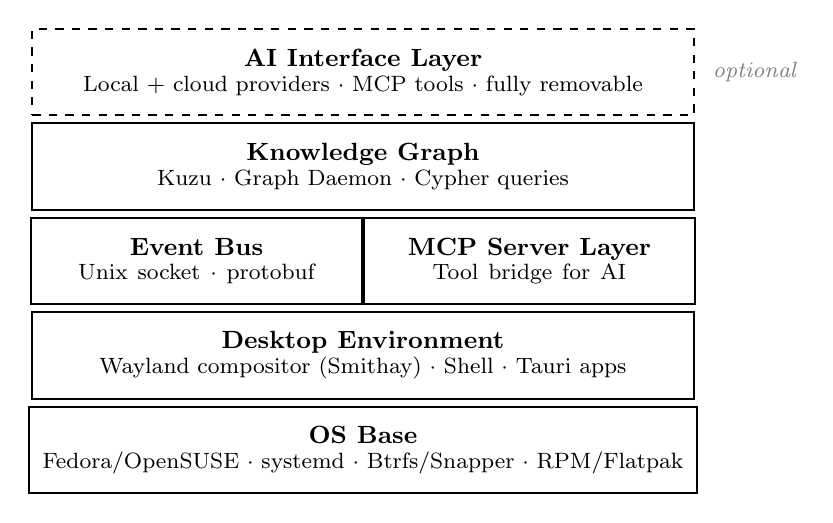
\begin{tikzpicture}[
  box/.style={
    draw, thick, rectangle,
    minimum width=8.4cm, minimum height=1.1cm,
    font=\small\bfseries, align=center, inner sep=5pt
  },
  optbox/.style={
    draw, thick, dashed, rectangle,
    minimum width=8.4cm, minimum height=1.1cm,
    font=\small\bfseries, align=center, inner sep=5pt
  },
  splitbox/.style={
    draw, thick, rectangle,
    minimum width=4.2cm, text width=3.8cm, minimum height=1.1cm,
    font=\small\bfseries, align=center, inner sep=5pt
  },
]

\def\sep{1.2}

\node[box] (os) at (0, 0) {
  OS Base\\[-2pt]
  {\mdseries\footnotesize Fedora/OpenSUSE $\cdot$ systemd $\cdot$ Btrfs/Snapper $\cdot$ RPM/Flatpak}
};
\node[box] (de) at (0, \sep) {
  Desktop Environment\\[-2pt]
  {\mdseries\footnotesize Wayland compositor (Smithay) $\cdot$ Shell $\cdot$ Tauri apps}
};
\node[splitbox, anchor=east] (eb) at (0.0, 2*\sep) {
  Event Bus\\[-2pt]
  {\mdseries\footnotesize Unix socket $\cdot$ protobuf}
};
\node[splitbox, anchor=west] (mcp) at (0.0, 2*\sep) {
  MCP Server Layer\\[-2pt]
  {\mdseries\footnotesize Tool bridge for AI}
};
\node[box] (kg) at (0, 3*\sep) {
  Knowledge Graph\\[-2pt]
  {\mdseries\footnotesize Kuzu $\cdot$ Graph Daemon $\cdot$ Cypher queries}
};
\node[optbox] (ai) at (0, 4*\sep) {
  AI Interface Layer\\[-2pt]
  {\mdseries\footnotesize Local + cloud providers $\cdot$ MCP tools $\cdot$ fully removable}
};
\node[font=\footnotesize\itshape, gray, anchor=west]
  at ([xshift=3pt] ai.east) {optional};

\end{tikzpicture}
\caption{System layer structure. Each layer depends only on the layer directly
below it. The AI Interface Layer is dashed to indicate it is fully optional and
can be disabled without affecting any other layer.}
\label{fig:layers}
\end{figure}

\subsection{Layer Responsibilities}
\label{sec:layer-responsibilities}

\paragraph{OS Base.}
The foundation is a standard Linux distribution providing the kernel, init
system, package manager, and base userspace tools. Nothing at this layer is
custom-built. The system builds on top of it; it does not replace it. The choice
of base distribution, the update strategy, and the concrete packages involved
are covered in detail in Section~\ref{sec:foundation}.

\paragraph{Desktop Environment.}
The Wayland compositor and the shell sit at this layer. This is what the user
directly interacts with: windows, the taskbar, the Spotlight launcher,
notifications, and the lock screen. All user-facing applications in this project
are built with \emph{Tauri}, a framework described in
Section~\ref{sec:tauri-intro}. The compositor itself is built on
\emph{Smithay}, described in Section~\ref{sec:smithay-intro}.

\paragraph{Event Bus.}
The internal message bus handles all communication between custom system
components. It receives, validates, and routes structured events from kernel
monitoring, the display system, and first-party applications. It runs as a
background service over \emph{Unix sockets} (see Section~\ref{sec:unix-sockets})
using \emph{Protocol Buffers} for schema-enforced serialization (see
Section~\ref{sec:protobuf}). Its role is purely to move and validate data; it
does not interpret or store anything.

\paragraph{MCP Server Layer.}
The \emph{Model Context Protocol} (MCP) is an open standard published by
Anthropic in 2024 for exposing application capabilities as callable tools that
AI models can invoke. Before MCP, every AI integration was bespoke: one
application called the OpenAI API in one format, another used a different
tool-calling convention, and combining them required custom glue code on both
ends. MCP standardizes this at the protocol level so that any MCP-compatible AI
client can communicate with any MCP server without application-specific
integration work. In this system, first-party applications expose MCP servers as
part of their standard implementation, giving the AI layer a structured,
permission-gated way to act on the system. The same interfaces are available to
any MCP-compatible client, not only the built-in AI layer.

\paragraph{Knowledge Graph.}
The graph database is the system's long-term memory. It stores events arriving
from the Event Bus as typed nodes and relationships, making it possible to query
across time, application boundaries, and data types. The \emph{Graph Daemon} is
the sole reader and writer of the underlying database; no other component
accesses the database file directly. Why a graph database rather than a
relational one, and why \emph{Kuzu} specifically, is explained in
Section~\ref{sec:kg-rationale}.

\paragraph{AI Interface Layer.}
The top layer provides AI capabilities to the rest of the system. It queries the
Knowledge Graph for context, exposes tools via the MCP layer, and mediates
between user requests and AI model providers. All providers, whether a local
model running on the device or a remote cloud API, are interchangeable behind a
common interface defined as a \emph{Rust trait} (see
Section~\ref{sec:rust-intro}). This layer is entirely optional: disabling it
removes AI features and nothing else.

\subsection{Why Rust}
\label{sec:rust-intro}

All system daemons and Tauri application backends in this project are written in
\emph{Rust}, a systems programming language developed by Mozilla Research with
its 1.0 release in 2015. Understanding why requires a brief look at what systems
programming has historically looked like.

C and C++ have dominated operating system components, daemons, and
performance-critical software for decades. Their advantage is direct control
over memory and hardware with minimal overhead. Their liability is that this
control is entirely manual: the programmer allocates memory and is responsible
for freeing it correctly, without using it afterward, without reading past its
bounds, and without sharing it unsafely across threads. Memory safety bugs ---
use-after-free, buffer overflows, data races --- are the single largest source
of exploitable vulnerabilities in system software. Google's Project Zero and
Microsoft's Security Response Center have independently reported that roughly
70\% of serious security vulnerabilities in their codebases are memory safety
issues~\cite{msrc2019memory}.

Go is a more recent alternative with garbage collection and a simpler
concurrency model, but its garbage collector introduces unpredictable pause
latency unsuitable for low-level system components, and its runtime overhead is
significant compared to C or Rust.

Rust enforces memory safety through a compile-time ownership and borrowing
system. An entire class of bugs that would be exploitable vulnerabilities in C
simply cannot compile in Rust --- the compiler rejects them. This is not a
runtime check with performance overhead; it is a zero-cost compile-time
guarantee. Rust has no garbage collector and achieves performance comparable to
C and C++.

For this project the consequence is concrete: every daemon runs continuously,
handles untrusted input from applications, and manages sensitive data including
credentials and graph queries. Writing them in Rust eliminates an entire
vulnerability class without sacrificing performance.

A \emph{Rust trait} is the language's mechanism for defining a shared interface
that multiple concrete types can implement --- analogous to an interface in Java
or a pure abstract class in C++. When this document refers to the AI provider
abstraction as a Rust trait, it means that every AI backend implements the same
set of methods, and the rest of the codebase calls only those methods without
knowing which concrete backend is active at runtime.

\subsection{Why Wayland}
\label{sec:wayland-intro}

\emph{Wayland} is a display server protocol: the specification that defines how
applications communicate with the component responsible for drawing windows on
the screen.

\emph{X11} (the X Window System) was designed in 1984 and has been the
foundation of graphical Linux desktops ever since. Its architecture reflects its
era: the display server is a separate process, and by default any application
can inspect the input events and window contents of any other application on the
same display. One X11 application can read keystrokes typed into another
application's window. This is a keylogger-class capability that cannot be
removed without a protocol redesign, and it makes X11 structurally incompatible
with the isolation guarantees this project requires.

Wayland redesigns this from scratch: each application communicates only with the
compositor, not with other applications. Input events are delivered only to the
window that currently has focus. An application cannot read another
application's keystrokes or window contents. This isolation is the default
behaviour, not an optional hardening measure.

Wayland also has a cleaner model for multi-monitor and HiDPI configurations:
each output carries its own scale factor, and applications receive this
information directly and render at the correct resolution automatically.

The compatibility cost is real. Wayland addresses it through \emph{XWayland},
an X11 compatibility server that runs as a Wayland client. Legacy X11
applications work inside XWayland without modification. X11's security
limitations apply within the XWayland boundary but are contained there and do
not affect native Wayland applications.

\subsection{Why Tauri}
\label{sec:tauri-intro}

\emph{Tauri} is a framework for building desktop applications with a Rust
backend and a web-based user interface. A Tauri application consists of a Rust
process that handles system interactions, file access, and IPC, and a
\emph{WebView} that renders the UI using standard web technologies: HTML, CSS,
and TypeScript. The two halves communicate through a typed command bridge: the
frontend calls Rust functions via \texttt{invoke()}, and Rust pushes events to
the frontend via Tauri's event emitter. No ad-hoc serialization is needed; the
bridge handles it.

The dominant alternative is \emph{Electron}, which takes the same split but
bundles an entire Chromium browser and a Node.js runtime with every application.
A minimal Electron application ships roughly 150\,MB of runtime dependencies and
consumes around 300\,MB of RAM at idle. On a system with several Electron
applications running, the memory cost is substantial.

Tauri uses the operating system's existing WebView implementation instead of
bundling one. On Linux this is \emph{WebKitGTK}, the GTK port of the WebKit
rendering engine. WebKitGTK is already present on any modern Linux desktop; a
Tauri application does not add it. A Tauri application binary is typically
5--10\,MB and uses a fraction of the RAM that an equivalent Electron application
would require.

Building the UI in a native toolkit such as \emph{GTK4} or \emph{Qt} was
considered and rejected for two reasons. First, maintaining visual consistency
across components developed independently is significantly harder with a native
toolkit than with a shared CSS design system where a token change propagates
everywhere. Second, the developer pool for TypeScript and CSS is larger than
for GTK or Qt development, which matters for an open-source project expecting
community contributions. The trade-off is that WebView rendering is slightly
less efficient than native rendering for highly dynamic content, but this is not
a relevant concern for the settings panels, file browsers, and launchers that
make up this system's UI.

Tauri version 2.0, released in October 2024, is used throughout this project.
Version 2.0 introduced a revised permission system for Tauri commands (replacing
the allowlist model of 1.x with a finer-grained capability model), official
mobile support, and improved IPC ergonomics. The capability model in 2.0 aligns
well with this project's general approach to least-privilege permissions.

\subsection{Why Smithay}
\label{sec:smithay-intro}

\emph{Smithay} is a Rust library for building Wayland compositors. It provides
the low-level plumbing: Wayland protocol handling, DRM/KMS interfaces for direct
display hardware access, input processing via \emph{libinput}, and buffer
management. Compositor logic such as window placement, focus rules, and workspace
behaviour is built on top of Smithay rather than dictated by it.

The alternative is \emph{wlroots}, a C library used by compositors including
Sway and Hyprland. wlroots is mature and widely deployed, but integrating it
into a Rust codebase requires C FFI (Foreign Function Interface) bindings, which
partially undermines the memory safety argument for using Rust: the boundary
between Rust and C code requires \texttt{unsafe} blocks that the Rust compiler
cannot verify. Smithay is written in Rust and integrates cleanly with the rest
of the codebase without unsafe boundaries.

The \emph{COSMIC} desktop from System76 is a production Rust-first Linux desktop
with comparable technical goals and uses Smithay as its compositor foundation.
It serves as a useful reference for what a Smithay-based desktop looks like in
practice.

\subsection{Component Boundaries}
\label{sec:component-boundaries}

The system's components divide into two categories: background services and
user-facing applications.

Background services are called \emph{daemons} in Unix terminology: processes
with no visible window that are started at boot by \emph{systemd} and
automatically restarted if they crash. systemd is the standard init system and
service manager on modern Linux distributions. It handles starting services in
dependency order at boot, logging their output to the journal, and enforcing
resource and sandboxing constraints via its service unit configuration. All
daemons in this project are written in Rust and run under tight systemd
sandboxing: each service unit declares exactly the filesystem paths, syscalls,
and network access it requires, and everything else is denied at the kernel
level.

\begin{table}[htbp]
\caption{Background services (daemons)}
\label{tab:daemons}
\begin{tabularx}{\linewidth}{lX}
\toprule
\textbf{Service} & \textbf{Responsibility} \\
\midrule
Event Bus       & Receives, validates, and routes internal events between components \\
Graph Daemon    & Sole reader/writer of the Knowledge Graph database \\
Account Daemon  & Credential management and login token handling \\
AI Layer Daemon & Runs AI models, coordinates tools, queries the graph \\
Module Runtime  & Manages the lifecycle of shell extensions \\
Transfer Daemon & Controls data movement between user profiles \\
Audit Daemon    & Sole writer to the append-only audit log \\
Health Daemon   & Aggregates and stores health and wellbeing data \\
Compositor      & Draws windows and manages the display (Wayland compositor) \\
\bottomrule
\end{tabularx}
\end{table}

User-facing applications are built with Tauri. Every first-party application
is built on two shared libraries. \emph{ui-kit} is a TypeScript component
library based on \emph{shadcn/ui} (a set of accessible, unstyled components
built on Radix UI primitives) styled with the project's shared design token
system using \emph{Tailwind CSS}. Tailwind is a utility-first CSS framework
where styles are applied via class names rather than separate stylesheets;
combined with CSS custom properties for design tokens, a theme change propagates
to all running applications without a reload. \emph{os-sdk} is a Rust crate that
provides ready-made clients for the Graph Daemon and Event Bus, MCP server
boilerplate, and the shared TOML configuration system. A new first-party
application starts with these two libraries and has graph access, event
emission, an MCP server, and a consistent UI without writing any infrastructure
code.

\begin{table}[htbp]
\caption{User-facing applications}
\label{tab:apps}
\begin{tabularx}{\linewidth}{lX}
\toprule
\textbf{Application} & \textbf{Notes} \\
\midrule
Shell        & Taskbar, Spotlight launcher, notification center, lock screen \\
Settings     & System-wide configuration: theming, permissions, AI level, accounts \\
File Manager & First-party file browser with graph-aware features \\
Store        & App and module discovery, installation, and updates \\
Terminal     & First-party terminal emulator with MCP integration \\
Wine Manager & Windows compatibility management UI \\
\bottomrule
\end{tabularx}
\end{table}

\subsection{Communication Model}
\label{sec:communication}

\subsubsection{Unix Sockets}
\label{sec:unix-sockets}

All inter-component communication uses \emph{Unix domain sockets}, a
communication mechanism built into the Linux kernel. A Unix socket behaves
like a network socket in its API but exists only on the local machine: it is
represented as a file path in the filesystem (for example
\texttt{/run/graph-daemon/graph.sock}), and only processes on the same machine
can connect to it. There is no network stack involved; data passes directly
through the kernel with latency in the range of a few microseconds.

D-Bus, the standard Linux IPC mechanism discussed in
Section~\ref{sec:dbus}, was not chosen for internal component communication:
it introduces a central broker process as an intermediary, adds marshalling
overhead, and its type system is not well suited to the structured binary
messages used here. TCP loopback sockets were also considered and rejected: they
go through the full network stack, carry more overhead, and expose a port
reachable by any process on the machine.

\subsubsection{Protocol Buffers}
\label{sec:protobuf}

Data transmitted over the internal sockets is serialized with \emph{Protocol
Buffers} (protobuf), a binary serialization format developed and open-sourced by
Google. Serialization is the process of converting a data structure in memory
into a byte sequence for transmission, and deserialization is the reverse.

The alternative most developers reach for is JSON, a human-readable text format.
JSON has two disadvantages for a high-frequency internal bus. First, it carries
no schema: any JSON object is syntactically valid, so a receiver cannot
distinguish a malformed message from a valid one without application-level
checks. Second, text encoding is inefficient: a 64-bit integer written as its
decimal string representation takes 1--20 bytes; protobuf encodes the same value
in 1--10 bytes using variable-length encoding.

Protobuf defines message types in \texttt{.proto} schema files, which are
compiled to Rust code. A message that does not match the schema is rejected by
the generated parser before it reaches application logic, catching schema
violations at the boundary rather than deep inside a handler.

\emph{MessagePack} was considered as an alternative: it is a binary JSON
variant with compact encoding but no schema enforcement. \emph{Cap'n Proto} and
\emph{FlatBuffers} offer zero-copy deserialization and faster parsing for large
messages, but their Rust ecosystems are less mature than protobuf's. Protobuf
has the best combination of schema enforcement, Rust library quality, and
tooling.

\begin{table}[htbp]
\caption{Inter-component communication paths}
\label{tab:comms}
\begin{tabularx}{\linewidth}{lX}
\toprule
\textbf{Path} & \textbf{Transport} \\
\midrule
Daemon $\leftrightarrow$ Daemon            & Unix socket (protobuf) \\
App backend $\leftrightarrow$ Daemon       & Unix socket (protobuf) \\
App backend $\leftrightarrow$ App frontend & Tauri command bridge (typed) \\
Compositor $\leftrightarrow$ Shell         & Wayland protocols + Unix socket \\
\bottomrule
\end{tabularx}
\end{table}

A concrete example: a user action in the UI that queries the Knowledge Graph
follows this path:

\begin{center}
\texttt{UI event $\to$ App backend $\to$ Unix socket $\to$ Graph Daemon $\to$ Database}
\end{center}

Four steps, all local to the machine. The full round-trip is imperceptible to
the user.

\subsubsection{Knowledge Graph Rationale}
\label{sec:kg-rationale}

A relational database such as \emph{PostgreSQL} or \emph{SQLite} organizes data
into tables with rows and columns. Relationships between entities are expressed
as foreign key references and queried using \texttt{JOIN} operations, which
become progressively more expensive and harder to write as the number of hops
between entities increases.

A \emph{graph database} stores relationships as first-class data: entities are
\emph{nodes} and the connections between them are typed \emph{edges}, both with
their own properties. Traversing a relationship is a direct pointer follow,
not a table scan or index lookup. Querying "which files did the user work on
last Tuesday, via which applications, and are any of those applications still
running?" is a single graph traversal. In SQL it requires at minimum three joins,
a time-range filter, and a correlated subquery for the running-process check.

For an operating system where everything is connected --- processes open files,
files belong to projects, projects span sessions, sessions involve multiple
applications --- a graph is the natural data model.

\emph{Kuzu} is the specific graph database used here. It is an embedded graph
database written in C++ with first-class Rust bindings, released under the MIT
license. \emph{Embedded} means it runs as a library inside the Graph Daemon
process with no separate server process, no network port, and no additional
service to manage. The database is a directory of files on disk that only the
Graph Daemon process opens.

\emph{Neo4j} was evaluated and rejected. Neo4j is the most widely deployed
graph database and has a large ecosystem, but it runs as a separate server
process, its community edition has usage restrictions, and its JVM-based runtime
carries memory overhead inappropriate for a component embedded in a user session.
SQLite with recursive Common Table Expressions for graph traversal was also
considered; the query complexity and traversal performance for deep graphs made
it unsuitable.

Kuzu uses \emph{Cypher} as its query language, an open graph query standard
(openCypher) originally developed for Neo4j. It reads close to natural language:

\begin{lstlisting}[language={}]
MATCH (f:File)-[:OPENED_BY]->(a:App)
WHERE f.last_modified > datetime('2026-03-01')
RETURN f.path, a.name
ORDER BY f.last_modified DESC
\end{lstlisting}

This query finds all files modified after a given date, which applications
opened them, and returns the results sorted by modification time.

\subsection{D-Bus Coexistence}
\label{sec:dbus}

\emph{D-Bus} is the standard inter-process communication system on Linux
desktops, in use since 2003. NetworkManager uses it to report network state
changes, BlueZ uses it for Bluetooth events, \texttt{systemd-logind} uses it
for session management, and the \emph{XDG Desktop Portal} uses it to give
sandboxed applications access to OS-level dialogs. It cannot be removed without
breaking the wider Linux software ecosystem.

D-Bus works as a message broker: a central \texttt{dbus-daemon} process routes
messages between senders and registered receivers identified by well-known bus
names such as \texttt{org.freedesktop.NetworkManager}. This model works well for
the ecosystem-level events it was designed for. The central broker and its
overhead make it a poor fit for the high-frequency structured events between
project-internal components, which is why the project uses its own Event Bus for
internal communication.

This system does not replace D-Bus. It runs alongside it. D-Bus remains
responsible for third-party application notifications via
\texttt{org.freedesktop.Notifications}, hardware events, portal interfaces, and
session management. The internal Event Bus handles communication between
project components only. The two systems are parallel and non-overlapping.

The rule for developers is simple: project-internal components communicate over
the internal Event Bus via Unix sockets and protobuf. Standard Linux services
and third-party applications communicate over D-Bus as they always have. No
component spans both buses.
